\documentclass[9pt]{amsart}
%\documentclass[10pt]{article}
\usepackage{xcolor}
\usepackage{tikz}
\usepackage[utf8]{inputenc}
\begin{document}
EXERCICES\newline\newline
Exercice 6 page 17\newline
Le croisement de deux lignes ne suffit pas pour faire une r\'{e}gion ferm\'{e}e, il faut au minimum trois lignes, la plus petite r\'{e}gion ferm\'{e}e est alors un triangle \newline
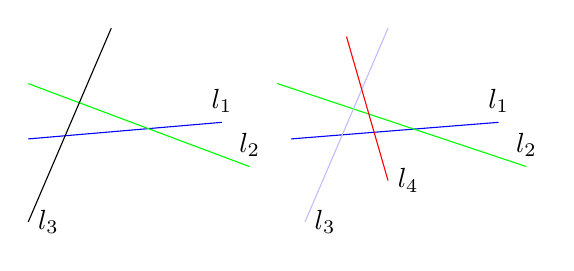
\begin{tikzpicture}
	\draw[color=blue] (0pt, 0pt) -- (70pt, 6pt) node[anchor = south, color=black] {$l_1$}; 
	\draw[color=green] (0pt, 20pt) -- (80pt, -10pt) node[anchor = south, color=black] {$l_2$}; 
	\draw (30pt, 40pt) -- (0pt, -30pt) node[anchor = west] {$l_3$}; 
	\draw[color=blue] (95pt, 0pt) -- (170pt, 6pt) node[anchor = south, color=black] {$l_1$};
	\draw[color=green] (90pt, 20pt) -- (180pt, -10pt) node[anchor = south, color=black] {$l_2$};
	\draw[color=blue!25] (130pt, 40pt) -- (100pt, -30pt) node[anchor = west, color=black] {$l_3$};
	\draw[color=red] (115pt, 37pt) -- (130pt, -15pt) node[anchor = west, color=black] {$l_4$};
\end{tikzpicture}\newline
Sur le sch\'{e}ma de gauche on a une r\'{e}gion ferm\'{e}e, un triangle, qui d\'{e}coule des intersections des trois lignes et sur le sch\'{e}ma de droite, compos\'{e} des intersections de quatre lignes, la r\'{e}gion ferm\'{e}e de gauche n'apparaît plus. Elle est coup\'{e}e par la ligne $l_4$. Ceci montre que l'ajout d'une ligne impose de recalculer toutes les r\'{e}gions ferm\'{e}es. \newline
Une r\'{e}gion ferm\'{e}e c'est un triangle, toutes les r\'{e}gions ferm\'{e}es sont les couples de deux droites coup\'{e}es par la droite $l_n$ derni\`{e}rement ajout\'{e}e. \newline\newline
On pose l'hypoth\`{e}se que le nombre maximum de r\'{e}gions ferm\'{e}es, obtenues  par les insertections de n droites, est :  $\binom{2}{n-1},  n\geq3$. \newline\newline
L'hypoth\`{e}se se v\'{e}rifie pour les deux premiers cas $\binom{2}{2} = 1$ et $\binom{2}{3} = 3$ puisque ($l_1l_2l_4,\; l_1l_3l_4,\; l_2l_3l_4$). D\'{e}montrons que l'hypoth\`{e}se reste vrai au rang $n+1$.
Quand on a n lignes le nombre de r\'{e}gions ferm\'{e}es est $\binom{2}{n-1}$ selon l'hypoth\`{e}se de r\'{e}currence. Si une droite est ajout\'{e}e il faut recalculer toutes les r\'{e}gions ferm\'{e}es et une r\'{e}gion ferm\'{e}e est un triangle. 
Si nous avons n+1 lignes, tous les triangles seront form\'{e}s de toutes les combinaisons de 2 lignes 
venant des n premi\`{e}res lignes et de la derni\`{e}re ligne ajout\'{e}e. 
On aura alors $\binom{2}{n}$ r\'{e}gions ferm\'{e}es. Voil\`{a} qui confirme l'hypoth\`{e}se de r\'{e}currence et si une r\'{e}gion a plus de 3 côt\'{e}s
il s'agit du croisement de plusieurs triangles. 
 \newline\newline
Exercice 7 page 17 \newline
Puisque $H(n) = J(n+1) - J(n)$ ça entraine que $H(n) \neq 2$ car si $n+1 = 8$ alors $H(7) = J(8) - J(7) < 2$.\newline
On a montr\'{e} avec un contre-exemple que  $H(n) \neq 2$.
\newline\newline
RECCURENT PROBLEMS (Homework exercises)
\newline\newline
8. Solve the recurrence 
$Q_{0} = \alpha; \;\; Q_{1}= \beta;$\newline 
$Q_{n} = (1 + Q_{n-1}) / Q_{n-2}$, for $n > 1$
\newline Assume that $Q_{n}  \neq 0$ for all n $\geq 0$\newline\newline
Nous allons calculer les autres termes de la suite jusqu' \`{a} $Q_{7}$.\newline
$Q_{2} = \frac{1+\beta}{\alpha}$;\; $Q_{3} = \frac{\alpha+\beta+1}{\alpha\beta}$;\; $Q_{4}=\frac{\alpha+1}{\beta}\;$; $Q_{5}= Q_{0};\; Q_{6} = Q_{1}; Q_{7} = Q_{2}$ 
\newline\newline Suite \`{a} ces calculs on pose comme hypoth\`{e}se de r\'{e}currence que $Q_{n} = Q_{(n\bmod5)}$ pour tout $n \geq 5$. L'hypoth\`{e}se se v\'{e}rifie au rang 5, nous supposons qu'elle reste vraie jusqu'au rang n. On a $Q_{n+1} = \frac{1 + Q_{n}}{Q_{n-1}}$ et on va montrer que, en fonction de chaque valeur de $n+1\bmod5$ l'hypoth\`{e}se se v\'{e}rifie. \newline\newline
Si $n+1 = k.b + r$ alors $n = k.b + (r-1)$ \newline
Si $n = k.b$ alors $n-1 = (k-1).b + b - 1$\newline
ainsi si $n+1 \bmod 5 = 0$ alors $Q_{n+1} = \frac{\beta+\alpha+1}{\beta}\times\frac{\alpha\beta}{\alpha+\beta+1} = \alpha$\newline
Si $n+1 \bmod 5 = 4$ alors $Q_{n+1} = \frac{(\alpha+1)(\beta+1)}{\alpha\beta}\times\frac{\alpha}{1 + \beta} = \frac{\alpha+1}{\beta}\;$\newline
Si $n+1 \bmod 5 = 3$ alors  $Q_{n+1} = \frac{\alpha+\beta+1}{\alpha}\times\frac{1}{\beta} = \frac{\alpha+\beta+1}{\alpha\beta}\;$\newline
Si $n+1 \bmod 5 = 2$ alors  $Q_{n+1} = \frac{1+\beta}{\alpha}$\newline
Si $n+1 \bmod 5 = 1$ alors  $Q_{n+1} = (1 + \alpha)\times\frac{\beta}{1+\alpha} = \beta$\newline\newline

L'hypoth\`{e}se est v\'{e}rifi\'{e}e dans tous les cas du rang n+1.
\end{document}
